\documentclass[dvipdfmx]{beamer} % Beamerクラスを使用

% ---------------------------------
% プリアンブル(設定部分)
% ---------------------------------
\usepackage[utf8]{inputenc} % 日本語環境では適宜変更(例:\usepackage[dvipdfmx]{graphicx} なども必要)
\usetheme{metropolis} % 例としてテーマを設定(Boadilla, Madridなども人気)

\usepackage{graphicx}

\usepackage{tikz}
\usetikzlibrary{shapes, arrows.meta, positioning}
\tikzset{
  terminal/.style={rounded rectangle, draw=black, text centered, inner sep=0},
  process/.style={rectangle, draw=black, text centered, inner sep=0},
  if/.style={diamond, draw=black, text centered,aspect=2, inner sep=0}
}

\usepackage{listings, jvlisting}
\lstset{
  basicstyle={\ttfamily\small},
  keywordstyle={\color{blue}},
  commentstyle={\color{green}},
  stringstyle=\color{red},
  tabsize=2,
  lineskip=-2ex
  %% breaklines=true, %折り返し
}

\title{ソフトウェアシンセサイザーの制作}
\author{渡邉 陽平}

\begin{document}
\begin{frame}
  \maketitle
\end{frame}

\begin{frame}
  \frametitle{目次}
  \begin{itemize}
  \item 制作の背景と目的
  \item システムの設計と仕様
  \item 実装のプロセス
  \item 主な工夫
  \item 実装予定の機能
  \end{itemize}
\end{frame}

\begin{frame}
  \frametitle{制作の背景と目的}
  現代の音楽制作において、\textbf{\Large シンセサイザーは不可欠なツール。}\par
  しかし、\textbf{\LARGE ブラックボックス化しているという現状。}\par
  \vspace{0.5cm}
  本研究ではシンセサイザーの制作を通してその構造や音響合成の仕組みを理解することを目的とします。\par
\end{frame}

\begin{frame}
  \frametitle{システムの設計と仕様(1)}
  \alert{\large 音声出力部}
  \begin{itemize}
  \item 規格:C17
  \item 役割:pcm情報を音声としてスピーカーから出力する。
  \item 採用理由:入出力に関するライブラリが豊富であるため採用。
  \item 使用ライブラリ:PulseAudioクライアントライブラリ16.1\par(音声出力)
  \end{itemize}
\vspace{0.5cm}
  \alert{\large 音響合成部}
  \begin{itemize}
  \item 使用言語:Fortran 2003
  \item 役割:音響合成を行う。
  \item 採用理由:信号処理に最適化された言語特性から採用した。
  \item 使用モジュール:ISO\_C\_BINDING(C言語との連携)
  \end{itemize}
\end{frame}    

\begin{frame}
  \frametitle{システムの設計と仕様(2)}
  \alert{システムのフローチャート}\par
  \begin{center}
    \begin{tikzpicture}[scale=0.75]
      \path[draw, dotted](5, -1)--(5, 6);
      
      \node[terminal](start) at (7, 6){開始};
      \node[text centered](t1) at (3, 6.5){C言語};
      \node[text centered](t2) at (7, 6.5){Fortran};
      
      \draw[->](7, 5.7)--(7, 5.5)--(3, 5.5)--(3, 5.25);
      \node[process](p1) at (3, 5){PulseAudio等の起動};
      \draw[->](3, 4.75)--(3, 4.5)--(7, 4.5)--(7, 4.25);
      \node[process](p2) at (7, 4){設定からインスタンス生成};
      \draw[->](7, 3.75)--(7, 3.5);
      \node[process](p3) at (7, 3.25){楽譜から音響合成};
      \draw[->](7, 3)--(7, 2.75)--(3, 2.75)--(3, 2.5);
      \node[process](p4) at (3, 2.25){音声出力};
      \draw[->](3, 2)--(3, 1.75)--(7, 1.75)--(7, 1.5);
      \node[if](if1) at (7, 0.75){演奏終了条件};
      \draw[->](7, 0)--(7, -0.5);
      \draw[->](9, 0.75)--(9.5, 0.75)--(9.5, 3.25)--(9, 3.25);
      \node at (8, -0.25){真};
      \node at (10, 0.75){偽}; 
      \node[terminal](end) at (7, -0.75){終了};
    \end{tikzpicture}
  \end{center}
\end{frame}

\begin{frame}
  \frametitle{システムの設計と仕様(3)}
  \alert{減算式シンセサイザーの構造}\par
  \begin{center}
    \begin{tikzpicture}[y=1.5cm]
      \node[process](m1) at (0, 2){オシレータ};
      \draw[->](1, 2)--(1.725, 2);
      \node[process](m2) at (2.5, 2){フィルタ};
      \draw[->](3.25, 2)--(4.375, 2);
      \node[process](m3) at (5, 2){アンプ};
      
      \node[process](m4) at (2.5, 3){エンベロープ};
      \draw[->, dashed](2.5, 2.9)--(0, 2.2);
      \draw[->, dashed](2.5, 2.9)--(2.5, 2.2);
      \draw[->, dashed](2.5, 2.9)--(5, 2.2);
      \node[process](m5) at (2.5, 1){LFO};
      \draw[->, dashed](2.5, 1.1)--(0, 1.8);
      \draw[->, dashed](2.5, 1.1)--(2.5, 1.8);
      \draw[->, dashed](2.5, 1.1)--(5, 1.8);
    \end{tikzpicture}
  \end{center}
\end{frame}

\begin{frame}[fragile]
  \frametitle{実装のプロセス(1)}
  \alert{オシレータの実装}
  
  例: 矩形波生成のFortranコード
  \begin{lstlisting}[language={Fortran}]
  IMPLICIT NONE
  PURE FUNCTION OSC\_SQUARE(X)
    REAL, INTENT(IN)::X
    REAL::OSC\_SQUARE

    REAL::I

    I = X-AINT(X)

    IF(I < 0.5)THEN
      OSC\_SQUARE=1
    ELSE
      OSC\_SQUARE=-1
    END IF
  END FUNCTION OSC\_SQUARE 
  \end{lstlisting}
  
  \vspace{0.5em}
%%   後のコーディング時の便宜を図るため、一周を$2\pi$ではなく1としている。
\end{frame}

\begin{frame}[fragile]
  \frametitle{実装のプロセス(2)}
  \alert{C言語とFortranの連携}\par
  ISO\_C\_BINDINGモジュールを用いることでC言語で定義された手続きをFortranから呼び出すことが可能になる。
  例:\par
  \begin{lstlisting}[language={C}]
    int hoge_in_c(int n, int m){
      ...
      return x;
    }
  \end{lstlisting}
  \begin{lstlisting}[language={Fortran}]
    USE ISO_C_BINDING
    FUNCTION HOGE_IN_F(N, M) BIND(C,&
            &NAME='hoge_in_c')
      INTEGER(C_INT), INTENT(in)::N,M
      INTEGER(C_INT), INTENT(OUT)::HOGE_IN_F
    END FUNCTION HOGE_IN_F
  \end{lstlisting}  
%%   このようにCの手続きをFortranで参照することにより、この場合であればHOGE\_IN\_Fとして呼び出すことが出来る。\par
%%   void型の関数を参照する場合は、関数としてではなくサブルーチンとして参照する。
\end{frame}

\begin{frame}
  \frametitle{実装予定の機能(1)}
  \alert{フィルター}\par
%%   減算式シンセサイザーでは、オシレータの音から不要な周波数成分をカットし、音色を変化させる。\par
%%   本研究では、アナログ回路のシミュレーションを利用して実装を目指す。\par
  例:ローパスフィルタ\par
  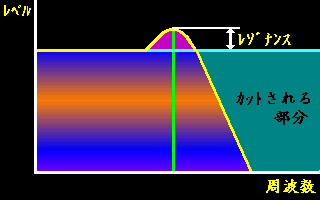
\includegraphics[scale=0.5]{lpf.png}\par
  \raggedleft{\footnotesize (出典:https://synth-voice.sakura.ne.jp/synth-voice/html5/synth-basic02.html)}  
\end{frame}

\begin{frame}
  \frametitle{実装予定の機能(2)}
  \alert{LFO}\par
%%   出力の大きさを周期的に変化させる。\par
%%   アンプに繋げばトレモロ、オシレータのピッチに繋げばビブラートが再現できる。\par
  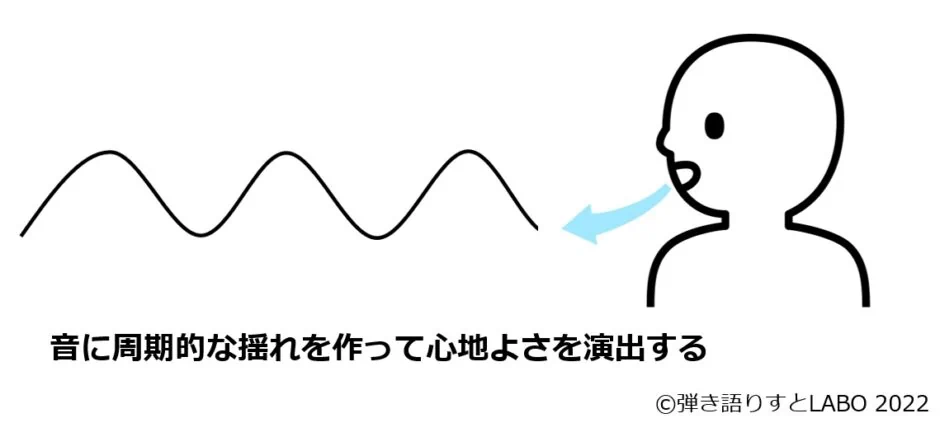
\includegraphics[scale=0.25]{vib.png}\par
   \raggedleft{\footnotesize (出典:https://hikigatarisuto-labo.jp/vibrato/)}  
\end{frame}

\begin{frame}
  \frametitle{実装予定の機能(3)}
  \alert{サンプリング周波数逓減モジュール}\par
%%   あえて波形をガタガタにすることで、レトロゲームのような効果を演出する。\par
  \begin{tikzpicture}[scale=0.6]
    \draw[->, very thick](0, 0)--(0, 3);
    \node at (-1, 3){出力};
    \draw[->, very thick](0, 1.5)--(6.5, 1.5);
    \node at (6.5, 1){時間};
    \draw[->, double, very thick](6.75, 1.5)--(7.25, 1.5); 
    \draw[->, very thick](8, 0)--(8, 3);
    \node at (7, 3){出力};
    \draw[->, very thick](8, 1.5)--(14.5, 1.5);
    \node at (14.5, 1){時間};
    
    \draw[thick](0, 1.5)--(1.5, 3)--(4.5, 0)--(6, 1.5);
    
    \draw[thick](8, 1.5)-|(8.5, 2)-|(9, 2.5)-|(9.5, 3)-|(10, 2.5)-|(10.5, 2)-|(11, 1.5)-|(11.5, 1)-|(12, 0.5)-|(12.5, 0)-|(13, 0.5)-|(13.5, 1)-|(14, 1.5);
  \end{tikzpicture}
\end{frame}
\end{document}
